% CSC501 Milestone 5: three-page semantic-layer report.
% Build: pdflatex main && bibtex main && pdflatex main && pdflatex main
\documentclass[sigconf,nonacm]{acmart}
\microtypesetup{expansion=false} % this build machine has no scalable CM fonts
\usepackage{xurl}
\settopmatter{printacmref=false,printfolios=true}
\setcopyright{none}
\renewcommand\footnotetextcopyrightpermission[1]{}
\acmDOI{}
\usepackage{array}
\usepackage{listings}
\usepackage{xcolor}
\urlstyle{same}
\graphicspath{{figures/}{../figures/}}
\raggedbottom
\emergencystretch=1em

\begin{document}

\title{Dated ETF Allocation Disclosures: A Semantic Layer over an Accepted Relational Model}
\titlenote{Project repository: \url{https://github.com/Pyrex111/CSC501_Data_Modeling_Project}}

\author{Taimoor Shahzad}
\affiliation{\institution{University of Victoria}\city{Victoria}\country{Canada}}
\author{M. Shahmeer Ather Kakwan}
\affiliation{\institution{University of Victoria}\city{Victoria}\country{Canada}}
\author{Mason Li}
\affiliation{\institution{University of Victoria}\city{Victoria}\country{Canada}}

\renewcommand{\shortauthors}{Taimoor et al.}

\begin{abstract}
The accepted Milestone 4 model records who holds which fund,
on which date, and what each provider disclosed about sector and geography,
with the capture it came from. This milestone adds a semantic layer: an OWL
ontology mirrors the twelve relations, aligns seven classes to FIBO, fixes
identity and provenance rules, and separates what OWL can state from what an
explicit validator must enforce. An embedded Oxigraph store holds the 356-triple
synthetic ABox beside the TBox; six SPARQL queries reproduce the accepted SQL
analyses, and a parity bridge and native validator gate every staged write. The
Flask interface now runs on the graph, sharing one validated instance across
search, detail, creation, batch update, deletion and portfolio views. The suite
passes 189 tests. Code and evaluation records: \url{https://github.com/Pyrex111/CSC501_Data_Modeling_Project}.
\end{abstract}

\keywords{ontology, OWL, RDF, FIBO, ETF, provenance, knowledge graph, data modelling}

\maketitle

\section{Introduction}
An exchange-traded fund allocation is a dated disclosure: a sector or geography
weight means little without the fund, the classification edition or captured
source, the as-of date and the document it came from. Milestone 4 delivered a
relational schema, a fully synthetic dataset and a Flask interface separating
customer holdings from provider disclosures and scoping categories by context.
Milestone 5 turns that model into a knowledge graph: Section~\ref{sec:ontology}
states the ontology and its FIBO boundary, Section~\ref{sec:backend} populates
the store, runs the six SPARQL analyses and keeps SQL/SPARQL parity, and
Section~\ref{sec:app} moves the interface onto the graph. All records are
fictional.

% Section 2 (ontology) of the Milestone 5 report. Owner: Mason Li.
% Written to be \input into the assembled main.tex. Numbers quoted here are
% checked against src/dal/sql/schema.sql and tests/test_semantic_ontology.py.

\section{Proposed Ontology}
\label{sec:ontology}

The accepted Milestone 4 model maps onto one ontology in two steps: each relation
becomes a class, and each column becomes a property. That baseline is applied
without shortcuts, and it accounts for the whole schema rather than a sample of
it. The schema has 51 non-identifier columns: 13 foreign keys and 38 scalar
columns. The keys collapse to 12 distinct forward object properties
(\texttt{hasDimension} serves both the snapshot and the category columns), and
five declared inverses complete the pairs, giving 17 object properties. The
scalar columns collapse to 36 distinct datatype properties, and one further
property, \texttt{recordId}, carries the surrogate row handle the application
still uses, giving 37 datatype properties. Twelve relations therefore yield
twelve classes.

\subsection{Classes, association classes and reused terms}

Two relations are association classes rather than link tables with a payload
attached: \texttt{Holding} carries a fractional interest and its own date, and
\texttt{AllocationEntry} carries the weight that belongs to a snapshot--category
pair. Both stay full classes. Collapsing either into a plain object property
would delete the very quantity the relation exists to hold.

Seven classes specialise FIBO\cite{fibo} or OMG Commons terms, shown in
Table~\ref{tab:alignment}: the portfolio and the holding reuse the FIBO ownership
classes, a snapshot is a \texttt{WeightedBasket} and an entry one of its
weighted constituents, and the scheme and the category reuse the FIBO fund
classification classes. Four published properties are reused as super-properties instead of being
invented: \texttt{weightFraction} is a sub-property of
\texttt{fibo:hasWeight}, both as-of columns are sub-properties of
\texttt{fibo:hasAsOfDate}, which FIBO explicitly distinguishes from a creation
date, and the two containment properties \texttt{hasEntry} and
\texttt{hasHolding} are sub-properties of the OMG Commons
\texttt{hasMember} and \texttt{comprises}. An allocation share is not a
fractional ownership interest, so no FIBO fractional-interest property is
claimed. The alignment is stated by IRI
only; the file carries no \texttt{owl:imports}, so it parses and validates offline
and the reuse stays an auditable claim rather than a network dependency.

% FIBO alignment table for Section 2. Owner: Mason Li.
% Local terms are in the etf namespace; inherited module paths are in
% milestones/05_semantic/docs/fibo_alignment.md.
\begin{table}[t]
\centering
\scriptsize
\caption{The reuse boundary. Seven classes specialise FIBO terms; five classes and
the observation attributes use project-specific definitions.}
\label{tab:alignment}
\begin{tabular}{@{}l@{}}
\toprule
\multicolumn{1}{@{}l}{\itshape reused (subsumption claim)}\\
etf:ETF $\sqsubseteq$ fibo:CollectiveInvestmentVehicle \\
etf:Portfolio $\sqsubseteq$ fibo:Portfolio \\
etf:Holding $\sqsubseteq$ fibo:Holding \\
etf:AllocationSnapshot $\sqsubseteq$ fibo:WeightedBasket \\
etf:AllocationEntry $\sqsubseteq$ fibo:WeightedBasketConstituent \\
etf:ClassificationScheme $\sqsubseteq$ fibo:FundClassificationScheme \\
etf:AllocationCategory $\sqsubseteq$ fibo:FundClassification \\
\midrule
\multicolumn{1}{@{}l}{\itshape extensions (no FIBO parent)}\\
Customer, ETFProvider (publisher role declined), ETFIdentifier, \\
AllocationDimension, SourceDocument (capture provenance) \\
\bottomrule
\end{tabular}
\end{table}


\subsection{Identity and context}

Identity is minted from the columns that already separate two records, never from
the surrogate \texttt{Id}, which is an artefact of row storage. Customers, providers,
dimensions and identifiers get \texttt{owl:hasKey}. Composite keys that name a
parent---a portfolio under a customer, a snapshot under a fund---do not: a
\texttt{hasKey} over an object property asserts individual equality across
parents, which is stronger than per-parent uniqueness. Those keys become URI
templates that mirror the constraint, one path segment per key component in key
order, with an explicit duplicate check beside them.

The category is the one class whose identity is not a single column. The schema
keys it by (dimension, context key, label). The context key is a prefix plus a
JSON list: either the classification authority, name and version, or --- when the
edition is unpublished --- the source URL, retrieval time, locator and dimension.
The graph reproduces that construction, and a parity test asserts that the graph
helper and the relational helper return byte-identical strings, so the two layers
cannot drift into disagreeing about which labels are the same label.

Provenance is structural, not annotational. Every snapshot keeps its source
document, its as-of date and the locator inside the capture that the weights were
read from, and the capture itself is retained by reference. An unresolved
classification edition keeps its version unrecorded instead of being assigned a
fabricated one, and a second unversioned edition for the same authority is
refused. Under the synthetic demonstration the retained file is generated, so the
file-existence check proves only that a capture exists---never that it supports
the numbers.

\subsection{What OWL states, and what it cannot}

The ontology states the schema's shape: domains and ranges, exactly-one and
at-least-one restrictions on participation, at-most-one scheme per category,
functional properties, four keys, and disjointness between snapshot, entry and
category. One axiom is worth singling out. The four schema triggers keep an
entry's category dimension equal to its snapshot's dimension; the graph restates
that as the property chain
\texttt{hasEntry}~$\circ$~\texttt{usesCategory}~$\circ$~\texttt{hasDimension}
$\sqsubseteq$~\texttt{hasDimension}.

But an open-world ontology\cite{owl2profiles} does not forbid what it does not
know, and it cannot add. A missing basis note is unknown, not invalid; a total of 0.94 against
\texttt{Complete} is not an axiom violation; a closed value set such as
\{Sector, Geography\} needs enumerated individuals, which would drag instance data
into the schema file. The dimension chain entails agreement but still cannot
\emph{flag} a disagreement, because without an \texttt{AllDifferent} assertion on
the dimension individuals the two dimensions may simply be the same individual.
Table~\ref{tab:split} records the split we ship: axioms for what must hold,
explicit checks for aggregation, closed sets, filesystem facts and composite
uniqueness. The validator module, built on RDFLib~\cite{rdflib}, publishes
both lists and a CLI, so the split can be reviewed without reading the code.

% OWL-versus-explicit rule split for Section 2. Owner: Mason Li.
\begin{table}[t]
\centering
\footnotesize
\caption{Where each accepted constraint is enforced. Four groups cannot be
axioms: aggregates, closed value sets, filesystem facts, and uniqueness that names
a parent.}
\label{tab:split}
\begin{tabular}{@{}>{\raggedright\arraybackslash}p{0.46\columnwidth}>{\raggedright\arraybackslash}p{0.50\columnwidth}@{}}
\toprule
Expressed as OWL/RDFS axioms & Requires an explicit check \\
\midrule
domains and ranges of all 54 properties & weights in $[0,1]$ \\
exactly-one participation, twelve functional properties & \texttt{Complete} total $=1\pm0.005$ (a sum) \\
at-most-one scheme per category & entry dimension $=$ snapshot dimension \\
\texttt{owl:hasKey} on four classes & closed sets: Sector/Geography, ISIN/Ticker, Complete/Partial/Unknown \\
property chain for dimension agreement & ISIN and ticker lexical shapes \\
disjointness of snapshot/entry/category & NOT NULL slots (open world reads absence as unknown) \\
FIBO subsumptions & context key against its scheme edition \\
 & composite keys that name a parent \\
 & capture file present inside the capture root \\
\bottomrule
\end{tabular}
\end{table}


The split is also the argument for the extension. FIBO's
\texttt{FundPortfolioInvestmentPolicy} describes how a portfolio is \emph{intended}
to be allocated; a snapshot records what a provider \emph{disclosed} on a date,
sometimes with partial coverage. Subsuming one under the other would license
inferences about managerial intent that the evidence does not support, so the
reuse stops at the basket and the constituent and the observation is modelled as
an extension with coverage status, basis note and locator. We likewise decline to
type the provider as FIBO's \texttt{Publisher} role: one relation plays both the
issuer and the publisher role, and the correct FIBO-shaped treatment would be two
role individuals over one party, a modelling change outside this milestone.


\begin{figure*}[t]
  \centering
  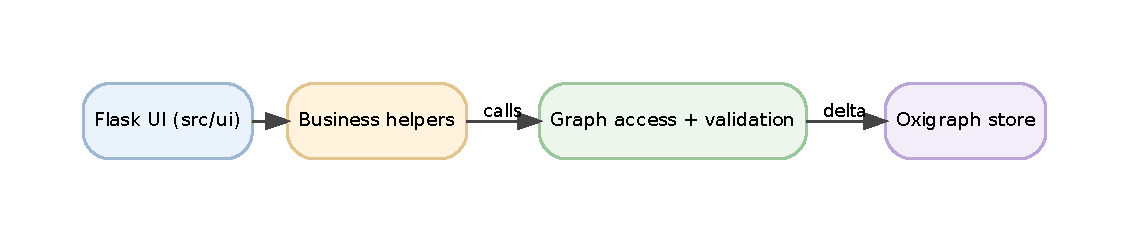
\includegraphics[width=\textwidth]{system_architecture_m5_wide.pdf}
  \caption{M5 flow: Flask UI, business helpers, graph access with validation
  before publish, and the embedded Oxigraph store holding separate ontology and
  data graphs.}
  \Description{Layered architecture: browser forms reach Flask routes, which
  call business helpers and graph repositories on one shared validated graph;
  rejected writes preserve the live store; the Oxigraph store keeps separate
  ontology and data named graphs.}
  \label{fig:architecture}
\end{figure*}

\section{Graph Population, SPARQL, and Reproducibility}
\label{sec:backend}
% Taimoor's AI-assisted M5 report contribution; executed evidence is documented
% in docs/taimoor_final_review.md and docs/taimoor_query_evidence.json.
Embedded Oxigraph stores twelve entity types as 356 fully synthetic instance
triples and loads the ontology into a separate named graph~\cite{oxigraphStore,oxigraphIO}.
Resource IRIs use \texttt{resource/\{Table\}/\{Id\}} as local record handles;
business uniqueness is validated separately. Relationships become IRI edges,
scalars typed literals, and unknown optional values are omitted. Holding and
allocation dates, classification context and captured-source provenance remain
distinct. Loading the ontology enables no OWL reasoner.

Six SPARQL SELECT queries reproduce the accepted SQL analyses. Complete result
multisets match, including duplicate multiplicity and unbound optional values;
row counts are 8, 2, 5, 5, 5 and 17. Numeric values are rounded to ten decimal
places for comparison. Q5 lists historical portfolio/disclosure candidates, not
a validated portfolio exposure total.

The following executable projection of Q3 counts and sums typed allocation
entries within each snapshot. Here \texttt{etf:} denotes the project ontology
namespace and \texttt{g:data} its data graph; the accompanying query file includes
both prefix declarations.
\lstinputlisting[firstline=4,basicstyle=\ttfamily\scriptsize,
  columns=fullflexible,keepspaces=true,breaklines=true,
  aboveskip=4pt,belowskip=4pt]{examples/taimoor_snapshot_totals.sparql}
\noindent The observed synthetic result is:
\begin{center}
\small
\begin{tabular}{@{}lrrrrr@{}}
\toprule
Snapshot \texttt{id} & 1 & 2 & 3 & 4 & 5 \\
\midrule
Entries \texttt{n} & 3 & 5 & 2 & 3 & 4 \\
Total fraction & 1.0 & 1.0 & 1.0 & 1.0 & 1.0 \\
\bottomrule
\end{tabular}
\end{center}
All five seeded snapshots are Complete. Grouping by the snapshot prevents
mixing disclosure dates, dimensions or blocks; class filtering prevents
\texttt{weightFraction} from including portfolio holdings. The SELECT reports
totals; write validation separately applies the prototype $0.005$ tolerance, without
forcing Partial or Unknown disclosures to total one.

Graph-backed CRUD stages each change on a candidate, runs the accepted M4
parity checks and Mason's native validator with capture-file checks, then
publishes one atomic SPARQL delta~\cite{sparqlUpdate}. Writers share one process
lock; rejected operations leave all live quads unchanged. No runtime inference
or ontology-graph lookup is needed on writes. Quickstart builds or reuses the
store and optionally starts Flask on the same graph instance. Verification
passed 189 tests; native-only rejection tests bypass the SQL bridge only inside
those tests. The six parity comparisons and the displayed query were also
executed on the same fresh seed. AI-executed checks are recorded separately from
student evaluation.


\section{Graph-Backed Application}
\label{sec:app}

% UI contribution for M5: Shahmeer (AI-assisted; reviewed by Shahmeer).
The M4 Flask interface now runs on the knowledge graph
(Figure~\ref{fig:architecture}). Users still search disclosures by ticker,
dimension and date, view source evidence, create disclosures, batch-edit
weights, delete entries and view dated portfolios, but they never write SPARQL.
At startup the integrated factory opens one shared graph, loads the ontology into
its own named graph and attaches both validators. The graph repositories keep the
M4 function signatures, result keys and error classes, so each route needed only
a data-access swap. Routes hold neither SQL nor SPARQL; the business layer still checks
dates, fractions, duplicate categories and empty forms.

Every write is staged on a candidate graph and published as one delta only after
validation. Rejected edits keep the user's input and show a plain message, and the business
layer translates validator messages such as duplicate snapshots, dimension
mismatches and unknown references. All 26 M4 route tests were rerun
unchanged against a fresh validated graph, and every rejection left the complete
quad set identical; with three new graph-specific tests the suite reaches 189
passing tests. A script rebuilds a throwaway graph and recaptures the eleven screenshots,
including the six write and rejection cases.

\paragraph{Evaluation and limits.}
A two-entry Complete snapshot (0.3, 0.7) rejects an edit to (0.1, 0.7), but
accepts the atomic batch (0.4, 0.6). Deleting a Partial entry succeeds; deleting
its final entry fails. Rejections preserve all quads, including the TBox, rather
than merely producing an error message. SQL parity verifies representation on
the seed, not real provider facts. The 0.005 tolerance is provisional, not measured
rounding error; synthetic captures exercise provenance, not independent financial
verification. One writable process is supported; no scalability or performance
claim follows from this demonstration.

% Architecture figure (full width):
% \begin{figure*}[t]
%   \centering
%   \includegraphics[width=\textwidth]{figures/system_architecture_m5.pdf}
%   \caption{M5 layers: Flask UI, business helpers, graph data access with
%   validation before publish, and the embedded Oxigraph store holding separate
%   ontology and data named graphs.}
%   \label{fig:architecture}
% \end{figure*}


\subsection{AI Assistance and Evaluation}
Two assistants were used. OpenAI ChatGPT/Codex~\cite{openaiAssistance} helped
draft ontology axioms, the validator, its documentation and part of the report
prose; Anthropic Claude~\cite{claudeAssistance} helped with the Flask routes and
UI tests, the architecture figure, cross-section consistency checks and this
revision. What matters is what they did, not which one: the 189 tests, the six
parity comparisons and the result table in Section~\ref{sec:backend} were
executed by the assistants on a fresh seed and are labelled AI-executed wherever
they appear, so none of them reads as a student-run evaluation. Design
decisions, the acceptance of each output and the final text remain ours: each
author reads and edits the sections attributed to him, and the Milestone 4
records keep human review apart from assistant-run checks. All data are synthetic.

\bibliographystyle{ACM-Reference-Format}
\bibliography{references}

\end{document}
